\subsection*{Viaje a Cornelia}
"¡Hasta la luna se cansa de dar vueltas esperando que muevan el trasero!"\\
\indent-- Cid 
\begin{center} 
	\tcbox[left=0pt,top=0pt,right=0pt,bottom=0pt, boxsep=0pt, colframe=accent, sharp corners]{
		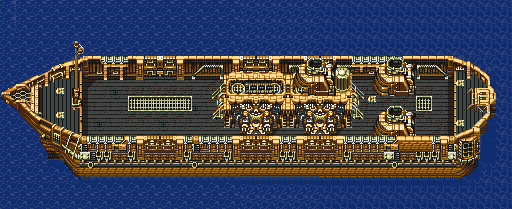
\includegraphics[width=0.98\columnwidth]{./art/maps/ship2.png} 
	}
\end{center}
La aventura comienza en un pequeño barco de transporte llamado "Pequeño Bronco", que está en camino de entregar carga a la ciudad de Cornelia. El capitán accedió a dejar que el grupo suba al barco por una pequeña tarifa. La tripulación del barco solo consta de 3 miembros: Biggs, Wedge y el capitán Cid. Los dos marineros llevan bandanas y pantalones cortos color celeste combinados con unas camisetas naranjas con rayas negras. Ambos son muy jóvenes e inexpertos, pero en general son amistosos con el grupo. No puede decirse lo mismo del viejo capitán, que se retiró a su camarote y prefiere que lo dejen solo. \subsubsection*{Día} "Aunque no lo parezca, soy todo un cobarde".\\
\indent-- Wedge \\\\
Si los aventureros no se conocen de antemano, deben presentarse primero, después de lo cual son libres de explorar el barco. También pueden hablar con los marineros que están felices de matar el tiempo durante el viaje. Biggs y Wedge les cuentan sobre recientes ataques piratas en altamar, que parecen haber aumentado recientemente. Además, también pueden darle al grupo novedades sobre Cornelia, ya que han oído que la princesa ha desaparecido. El grupo también puede preguntar sobre Cid, en cuyo caso los navegantes les cuentan su pasado como soldado. A medida que comienza a oscurecer, la tripulación se retira a sus cabinas. Los aventureros se preparan para terminar el día, cuando de repente se escuchan ruidos fuertes que rodean el barco. De inmediato se dan cuenta de que varios piratas han abordado al Pequeño Bronco. \subsubsection*{Batalla en el Pequeño Bronco} Coloca aproximadamente un pirata en el barco por cada miembro del grupo y distribúyelos alrededor de la plataforma como creas conveniente. La tripulación del barco está fuera de vista, luchando contra otros piratas que han entrado en el barco por debajo de la cubierta. Si las cosas se llegan a complicar para el grupo durante esta batalla, Biggs y Wedge pueden subir para ayudarlos. Sus detalles de combate se muestran a continuación. Son los mismos que los de los piratas. Después de derrotar a los enemigos, recuerda recompensar al grupo con el Gil que cada pirata derrotado dejó. Después de la batalla, la tripulación se reúne con el grupo y Cid les agradece su ayuda. Les explica que esta no es la primera vez que los atacan estos piratas, que son parte de la tripulación del capitán Bikke. Ahora, el grupo puede bajar a dormir para recuperar por completo sus PV y PM. Poco después de despertarse por la mañana, el barco llega a puerto de Cornelia. Una vez allí, la tripulación comienza a descargar la mercadería y se separa del grupo.
%
\vspace{0.5cm}
%
\monster{Pirate / Biggs / Wedge}{1}{
\includegraphics[width=0.16\textwidth]{./art/monsters/pirate.png}}
{
	HP: & \hfill 8 & MP: & \hfill 0\\
	STR: & \hfill 1 & DEF: & \hfill 0 \\
	MAG: & \hfill 0 & RES: & \hfill 0 \\
	AGI: & \hfill 3 & Size: & \hfill M\\
}
{
	\textbf{Scimitar}: 1d DMG \hfill \textbf{Drops:} 150 Gil 
}
%
\vspace{0.5cm}
%
\subsection*{Puerto de Cornelia}
El puerto de Cornelia es pequeño y tiene capacidad para un puñado de barcos de carga como el Pequeño Bronco. Los marineros del puerto están descargando cajas de los barcos, ya sea para almacenarlos en depósitos o llevarlos directamente a Cornelia. Luego de desembarcar, el grupo puede preguntar por el puerto cómo llegar a Cornelia. Los marineros les sugieren que tengan cuidado, ya que los guardias del castillo no están patrullando el camino. Cornelia no está lejos del puerto y el camino está rodeado principalmente de campos y prados.
%
\vfill
\tcbox[left=0pt,top=0pt,right=0pt,bottom=0pt, boxsep=0pt, colframe=accent, sharp corners]{
	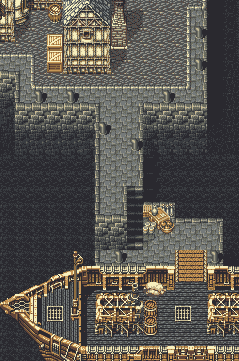
\includegraphics[width=0.98\columnwidth]{./art/maps/port.png} 
}
%
\subsubsection*{Dyce}
"Por cierto… ¿necesitan algo? ¡Echen un vistazo a mis productos! Es posible que se sorprendan con lo que encuentren..."\\
\indent-- Dyce \\\\
El grupo puede toparse en el puerto con un mercader errante llamado \textbf{Dyce}. Dyce es un hombre alto y fornido. Es calvo con barba y luce ropas oscuras. También tiene un \hyperlink{chocobo}{Chocobo} a su lado, que utiliza como medio de transporte. Le brinda información al grupo sobre los problemas de Cornelia, ya que ha oído rumores de que la princesa fue secuestrada. También vende Pociones a 125 Gil cada una, pero tiene más inventario que el grupo no puede permitirse en este momento. Dyce es un viajero, así que es probable que el grupo vuelva a encontrarse con él en el futuro. Sus precios suelen ser más altos en comparación con las tiendas habituales.

\subsubsection*{Batalla en el Puerto de Cornelia}
"¡Deben tener bolas de acero para desafiarme a mí!" -- Bikke \\\\
Al hablar con Dyce u otros marineros, el grupo se entera de que últimamente el puerto suele ser atacado por piratas. Normalmente el puerto está protegido por las guardias de Cornelia, pero desde la desaparición de la princesa, el rey ha replegado a todas las tropas al castillo. Los piratas siempre atacan por la noche y si grupo espera en los alrededores del puerto hasta que anochezca, en cualquier día, presenciaran un ataque de los piratas. Como el grupo lo sabe de antemano, pueden intentar adoptar medidas defensivas de antemano, como preparar una emboscada o trampas. El ataque comienza con un gran barco pirata que atraca en el puerto y varios piratas que despliegan para robar los depósitos y otros barcos. Los piratas son, una vez más, la tripulación del Capitán Bikke, pero esta vez también está presente el mismísimo Bikke. Durante la batalla, Bikke permanece detrás de las líneas ofensivas y se retira inmediatamente hacia su barco una vez que recibe cualquier daño. También hay algunos de sus hombres a su lado, de nuevo uno para cada miembro del grupo. Dado que es probable que Bikke escape de la batalla, el grupo puede volver a encontrarse con él en el futuro. Después de rechazar el ataque de los piratas, los marineros del puerto están muy agradecidos con el grupo y les ofrecen alojamiento y comida gratis por esa noche.
\vfill
\monster{Bikke}{2}{
\includegraphics[width=0.15\textwidth]{./art/monsters/pirate2.png}}
{
 PV: & \hfill 30 & PM: & \hfill 25\\
 FUE: & \hfill 1 & DEF: & \hfill 2 \\
 MAG: & \hfill 1 & RES: & \hfill 2 \\
 AGI: & \hfill 2 & Tamaño: & \hfill M\\
}
{
 \textbf{Cimitarra}: 1d de daño \mspell{Electro}{4}{0t}{Único}{3u}{Infliges 2d de daño \hyperlink{type}{Eléctrico} al objetivo}{\lightning} \mtech{Arenga}{5}{0t}{Único}{3u}{El objetivo recibe \hyperlink{status}{aumFUE} por 1 turno.}{\enstr} }

\clearpage